% Notes from the VO - Introductory Statistics
\documentclass[12pt, a4paper]{article}

\usepackage[utf8]{inputenc}
\usepackage[ngerman]{babel}

\usepackage{amsmath}        % Package for mathematical formulars and symbols
\usepackage{graphicx}       % Package for image imports

\graphicspath{ {./images/lecture1/} }
\setlength\parindent{0pt}   % No indentation for paragraphs

\title{Notizen der Vorlesung\\Einführende Statistik}
\author{Roberto Alfredo MezaMeza }
\date{Oktober 2024}

\begin{document}
\sloppy

\maketitle
\newpage

\section{Vorlesung 1}
    Übersicht zur Lehrveranstaltung und kleine Beispiele, inklusive eines Programmierbeispieles, für die Einleitung
    in die Vorlesung.

    \subsection{Das Ziegenproblem}
        Es gibt drei Türen, eine dieser Türen hat einen Preis dahinter versteckt. Bei diesem Gewinnspiel
        wird dann in dieser Reihenfolge vorgegangen:

        \begin{enumerate}
            \item Teilnehmer:in wählt eine Tür.
            \item Die Moderatorin weiß die Platzierung des Preises. Sie öffnet eine Tür die nicht gewählt wurde und die nicht den Preis entählt.
            \item Die oder der Teilnehmer:in bekommt die Möglichkeit zu Wechseln.
        \end{enumerate}

        Die Frage ist jetzt, soll gewechselt werden, oder nicht? Die Möglichkeit das Tor zu wechseln bedeutet, dass
        die oder der Teilnehmer:in die folgende Wahl hat:

        \begin{itemize}
            \item \textbf{Wahl A:} Tor 1 mit $P(Gewinn)=\frac{1}{3}$
            \item \textbf{Wahl B:} Tor 2 \underline{oder} Tor 3 mit $P(Gewinn)=\frac{2}{3}$
        \end{itemize}

        \begin{figure}[h]
            \centering
            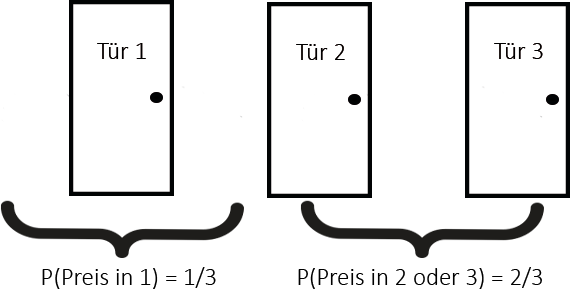
\includegraphics[width=0.5\textwidth]{monty-hall-problem_example}
            \caption{Eine visuelle Darstellung des Ziegenproblems}
        \end{figure}

\newpage

    \subsection{Statistik in KI und Data Science}
        KI und Data Science sind angewandte Statistik. Ein Beispiel sind Large Language Models (LLMs),
        wie ChatGPT.

        Wie auf Abbildung x dargestellt, iteriert dieses Verfahren. Das bedeutet, dass t' an das Prompt
        angehängt wird und der Prozess beginnt von vorne.

    \subsection{Vorlesungsmodalitäten}
        \begin{itemize}
            \item Inhalt, Abschriften und Ankündigungen auf Moodle.
            \item Literaturliste findet man auf Moodle. Die Vorlesung orientiert sich aber hauptsächlig an das Buch ``L. Wassermann, All of Statistics, Springer, 2005''
            \item Teilnahme an der Vorlesung nicht verpflichtend aber nachdrücklich empfohlen.
            \item Erster Prüfungstermin ist am 27.01.2025, im Zeitraum von 18:30 bis 21:00, Hörsaal 1, in der Währingerstraße 29.
            \item Anmeldung zur Prüfung erfolgt separat über UNIVIS Online oder u:space.
            \item Zur Prüfung muss ein Lichtbildausweis mitgenommen werden.
        \end{itemize}

\end{document}